\section{Resultados}
\label{sec:resultados}
% Todos los números de esta sección son del conjunto de PRUEBA (salvo que se aclare).

\subsection{Pre-procesamiento}

El canal azul es el que mejor separa la lesión de la piel en entrenamiento (AUC medio 0,976, seguido por $G$ con 0,965), porque la melanina absorbe más la luz azul, y $V$, propuesto en el anteproyecto, queda entre los peores (0,902). Por eso se segmenta sobre $B$, y el borde se sigue midiendo sobre $V$, donde interesa el cambio de brillo. Con el perfil radial de la viñeta, sólo 4 de las 200 imágenes pierden más del 2\,\% de la lesión (máximo 5,9\,\%). El filtro de forma de los pelos evita borrar la red, ya que en IMD200, sin pelos, el umbral solo marca como pelo el 28\,\% de la lesión y el filtro completo el 1\,\% (figura~\ref{fig:pelos} del anexo).

\paragraph{Hipótesis 1.} Se consideran con pelos las imágenes con más del 10\,\% de sus píxeles marcados, 30 de entrenamiento y 9 de prueba. La hipótesis no se confirmó (tabla~\ref{tab:h1}). En entrenamiento el cierre empeora más imágenes de las que mejora, con diferencia significativa sólo frente a la mediana, y en prueba no hay diferencia. El promedio de entrenamiento cae por cuatro imágenes que pierden más de 0,1 de Dice. En ellas el detector marca como pelo entre el 46 y el 78\,\% de la lesión, porque confunde la red y la textura oscura con pelos, y el \emph{inpainting} aclara la lesión, que M3 recorta. Se mantiene el cierre porque no suaviza la red que mide M5 y porque cambiarlo después de mirar prueba invalidaría la evaluación.

\begin{table}[!htb]
  \centering\small
  \begin{tabular}{@{}lccccc@{}}
    \toprule
    & \multicolumn{3}{c}{Dice medio} & \multicolumn{2}{c}{Cierre mejora / empeora (p)} \\
    Conjunto (imágenes) & Sin quitar & Mediana & Cierre & Frente a sin quitar & Frente a mediana \\
    \midrule
    Entrenamiento (30) & 0,893 & 0,898 & 0,873 & 10 / 20 (0,10) & 9 / 21 (0,025) \\
    Prueba (9) & 0,841 & 0,841 & 0,838 & 4 / 5 (0,65) & 3 / 6 (0,36) \\
    \bottomrule
  \end{tabular}
  \caption{Segmentación de las imágenes con pelos según cómo se quitan. El valor p es de la prueba de Wilcoxon.}
  \label{tab:h1}
\end{table}

\paragraph{Compresión.} A calidad 95 el archivo ocupa unas 8 veces menos, con un PSNR en la lesión de 40,7\,dB, un SSIM de 0,97 y un $\Delta E$ de 1,9, imperceptible (tabla~\ref{tab:compresion} del anexo). Desde calidad 75 el $\Delta E$ (2,7) supera el umbral de percepción, así que los colores en los que se basa C cambian de forma visible, y a calidad 10 el PSNR baja a 28,7\,dB, el SSIM a 0,70 y la red se reemplaza por bloques de $8\times8$ (figura~\ref{fig:compresion} del anexo).

\subsection{Segmentación}
\label{sec:res-segmentacion}
Los cinco métodos quedaron muy cerca en entrenamiento (tabla~\ref{tab:metodos} del anexo). Elegimos el crecimiento de regiones ($\sigma=4$\,px, tolerancia 0,5, apertura de 3\,px y cierre de 10\,px), que falla en una imagen menos que \emph{watershed} y es casi diez veces más rápido. Otsu y Chan-Vese tienen la mediana más alta, pero fallan en 6 y 7 imágenes, porque en las lesiones chicas el histograma casi no tiene pico de lesión y el umbral se corre hacia la piel.

En prueba, el crecimiento de regiones da un Dice medio de 0,916 y una mediana de 0,946, parecidos a los de entrenamiento. Encuentra el 82,8\,\% de los píxeles de lesión y marca como lesión sólo el 1,1\,\% de los de piel, así que su error típico es quedarse corto. Falla en 2 imágenes de prueba y 2 de entrenamiento, las 4 melanomas con azul grisáceo que dejó afuera (figura~\ref{fig:casos} del anexo), porque ese color refleja bastante luz azul y en $B$ se ve casi como la piel. Ningún método resolvió esos casos sin empeorar el resto.

\subsection{Criterios y comparación con el dermatólogo}
\paragraph{Asimetría.} El $\kappa$ con el dermatólogo es 0,44 en entrenamiento y 0,38 en prueba, con coincidencia exacta en el 67\,\% de las imágenes de prueba. Muchos desacuerdos aparecen porque el dermatólogo también mira cómo está repartido el pigmento, y el programa sólo mira la forma (figura~\ref{fig:asimetria} del anexo).

\paragraph{Borde.} El gradiente normalizado separó al revés de lo esperado (AUC entre 0,24 y 0,38), porque en PH2 los nevos comunes suelen tener borde nítido y los atípicos y melanomas, bordes que se desvanecen. Elegimos el gradiente crudo con umbral 0,0513, el único que suma en el sentido del TDS, aunque separa poco (AUC 0,60 en prueba).

\paragraph{Color.} El $\kappa$ de C es 0,17 en entrenamiento y 0,24 en prueba, aunque en el 80\,\% de las imágenes la diferencia es de un color como mucho. El marrón claro aparece en 42 de las 44 lesiones de entrenamiento donde no fue anotado, porque es el color del borde, y el blanco casi nunca, porque se asigna a la piel, mientras que el marrón oscuro, el azul grisáceo y el negro andan mejor ($\kappa$ entre 0,49 y 0,57 en prueba, figura~\ref{fig:colores} del anexo).

\paragraph{Circularidad y máscara manual.} La circularidad separa bien los grupos (AUC 0,72 en prueba), con mediana 0,34 en los melanomas y 0,71 en los nevos comunes. Con la máscara de PH2 los criterios no mejoran, ya que el $\kappa$ de A baja de 0,44 a 0,29 y el AUC de la circularidad de 0,75 a 0,57 en entrenamiento, así que los desacuerdos no vienen de la segmentación.

\paragraph{Estructuras.} Los detectores se mantienen en prueba (tabla~\ref{tab:estructuras}). Las estrías bajan de 0,79 a 0,67, con sólo 12 imágenes de prueba con estrías. La red atípica y los puntos y glóbulos, patrones finos, se detectan peor y con especificidad baja (0,46 y 0,44), así que el D estimado tiende a pasarse. El valor exacto de D acierta en el 27\,\% de las imágenes de prueba, menos que decir siempre la mediana de entrenamiento (50\,\%), con $\kappa=0{,}07$, porque basta errar una estructura para errar el valor.

\begin{table}[!htb]
  \centering\small
  \begin{tabular}{@{}lccc@{}}
    \toprule
    Estructura & Imágenes con la estructura & AUC entrenamiento & AUC prueba \\
    \midrule
    Red de pigmento atípica & 82 / 34 & 0,66 & 0,61 \\
    Puntos y glóbulos & 78 / 35 & 0,60 & 0,63 \\
    Estrías & 18 / 12 & 0,79 & 0,67 \\
    Regresión & 19 / 6 & 0,79 & 0,79 \\
    Velo azul-blanquecino & 24 / 12 & 0,95 & 0,93 \\
    \bottomrule
  \end{tabular}
  \caption{Detección de cada estructura de D. El AUC mide qué tan bien la medida separa las imágenes en que el dermatólogo marcó la estructura de las demás. Las cantidades son de entrenamiento y de prueba.}
  \label{tab:estructuras}
\end{table}

\subsection{Zonas y mapas de características}
Los atributos GLCM de toda la lesión no se sostienen en prueba (la correlación, el mejor, pasa de un AUC de 0,76 en entrenamiento a 0,62). La información no está repartida de manera pareja (figura~\ref{fig:mapas} del anexo). En entrenamiento, en los nevos comunes la mediana de la entropía baja de adentro hacia afuera (4,40 en el centro, 4,31 en la periferia y 4,16 en la interfase interna), y en las sospechosas esa caída no aparece (4,31, 4,40 y 4,33).

En prueba (tabla~\ref{tab:auc-prueba}), D estimado alcanza un AUC de 0,67 y la saturación de periferia menos centro, 0,71, pero sigue de cerca al brillo de la lesión ($\rho=-0{,}67$), que solo da un AUC parecido. La saturación de piel menos lesión queda en 0,60, con un intervalo que incluye al 0,5, y baja cuando M3 acierta más ($\rho=-0{,}42$ con el Dice), así que en parte mide errores de segmentación.

\begin{table}[!htb]
  \centering\small
  \begin{tabular}{@{}lccc@{}}
    \toprule
    Medida & AUC entrenamiento & AUC prueba & IC 95\,\% en prueba \\
    \midrule
    D del dermatólogo (techo) & 0,92 & 0,88 & 0,81 a 0,94 \\
    D estimado & 0,76 & 0,67 & 0,54 a 0,80 \\
    Periferia menos centro, $S$ & 0,76 & 0,71 & 0,58 a 0,84 \\
    Piel menos lesión, $S$ & 0,69 & 0,60 & 0,46 a 0,75 \\
    Oscuridad de la lesión ($-V$) & 0,75 & 0,68 & 0,54 a 0,80 \\
    \bottomrule
  \end{tabular}
  \caption{Capacidad de cada medida para separar lesiones sospechosas de nevos comunes (140 imágenes de entrenamiento y 60 de prueba).}
  \label{tab:auc-prueba}
\end{table}

\subsection{Clasificación}
El TDS automático separa las lesiones sospechosas de los nevos comunes con un AUC de 0,77 en prueba, con un intervalo que no incluye al 0,5, y la primera parte de la hipótesis 2 se confirma (tabla~\ref{tab:tds} y figura~\ref{fig:roc}). Por separado, los criterios que más aportan son A y C (AUC 0,73 y 0,69), seguidos por D (0,67) y B (0,60). El TDS extendido llega a 0,79, pero la diferencia con el TDS es de 0,02 y su intervalo ($-0{,}06$ a 0,09) incluye al cero, así que la segunda parte no se confirma. El umbral clínico resulta muy conservador, porque detecta sólo el 39\,\% de las sospechosas, mientras que el de Youden queda en 3,25 y equilibra mejor las dos medidas. Que sea más bajo es esperable, porque nuestro D parte de 0 y el borde automático suele dar valores bajos.

\begin{table}[!htb]
  \centering\small
  \begin{tabular}{@{}lcccc@{}}
    \toprule
    Clasificador & Umbral & Sensibilidad & Especificidad & AUC (IC 95\,\%) \\
    \midrule
    TDS, umbral clínico & 4,75 & 0,39 & 0,96 & 0,77 (0,65 a 0,89) \\
    TDS, umbral de Youden & 3,25 & 0,69 & 0,88 & 0,77 (0,65 a 0,89) \\
    TDS extendido, umbral de Youden & 3,49 & 0,72 & 0,75 & 0,79 (0,67 a 0,90) \\
    \bottomrule
  \end{tabular}
  \caption{Clasificación de las 60 imágenes de prueba en lesiones sospechosas y nevos comunes. Los umbrales de Youden se eligieron en entrenamiento.}
  \label{tab:tds}
\end{table}

\begin{figure}[!htb]
  \centering
  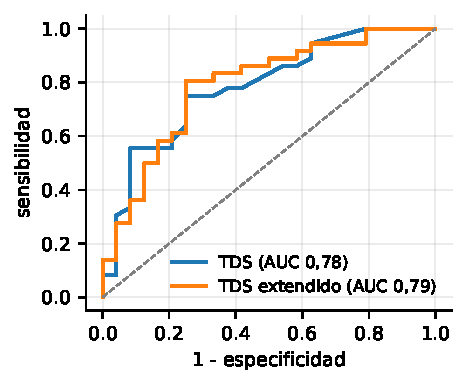
\includegraphics[width=0.42\textwidth]{m7_roc}\hspace{0.06\textwidth}
  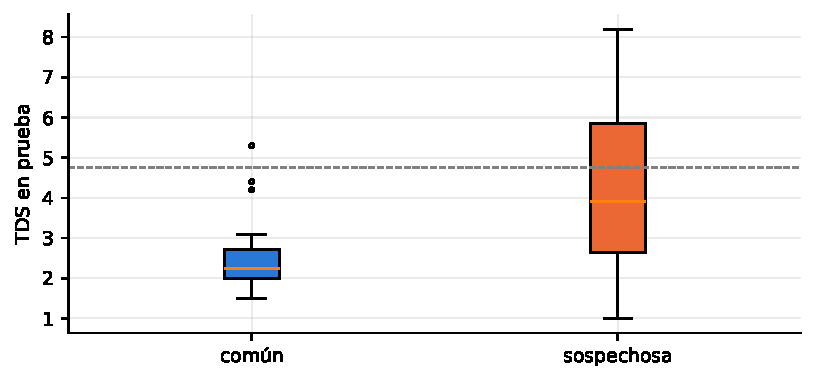
\includegraphics[width=0.42\textwidth]{m7_tds_grupos}
  \caption{Curvas ROC del TDS y del TDS extendido en prueba (izquierda) y distribución del TDS por grupo, con el umbral clínico en línea punteada (derecha).}
  \label{fig:roc}
\end{figure}
